% =============================================================================
% Section 4.8: Payment Module
% =============================================================================

\section{Payment Module}
\label{sec:payment-module}

\subsection{Functional Description}

The Payment module manages the lifecycle of financial transactions between learners and the platform. It integrates with Stripe for payment processing and webhook delivery, maintains its own payment intent state machine for reconciliation, and coordinates with the Enrollment module to activate course access only after successful payment. The module also handles refunds, partial payments, and coupon applications.

The module is designed to be Stripe-agnostic at the domain layer: the PaymentIntent aggregate and its state machine use a generic set of states and commands. A dedicated StripeInfrastructureService maps Stripe-specific constructs (PaymentIntent API objects, webhook event types) to the domain model, allowing the payment provider to be swapped without modifying domain logic.

\subsection{Stripe Integration and Webhook Handling}

Checkout flow proceeds as follows:

\begin{enumerate}
  \item The client requests \texttt{POST /api/payments/create-checkout} with course ID and learner ID. The Payment module creates a Stripe Checkout Session via the Stripe SDK and returns the session URL to the client.
  \item The client redirects the learner to Stripe's hosted checkout page. The learner completes payment on Stripe's domain, which reduces PCI-DSS compliance scope for the platform.
  \item Stripe sends a \texttt{checkout.session.completed} webhook to NexaLearn's \texttt{POST /api/payments/stripe-webhook}. The webhook handler verifies the Stripe signature using \texttt{stripe.webhooks.constructEvent()}, retrieves the session details, and invokes the \texttt{HandlePaymentSucceededUseCase}.
  \item The use case loads or creates a \texttt{PaymentIntent} aggregate, transitions it to SUCCEEDED, and publishes a \texttt{PaymentSucceeded} outbox event. The Enrollment module's event handler creates or activates the corresponding enrollment.
\end{enumerate}

Webhook idempotency is critical---Stripe may deliver the same webhook event multiple times. Stripe events include a unique \texttt{idempotency\_key} in their HTTP header; NexaLearn records processed webhook IDs in a ledger table and ignores duplicates:

\begin{lstlisting}[caption=Idempotent Stripe Webhook Processing,label=lst:stripe-idempotent]
async function handleWebhook(event: Stripe.Event): Promise<void> {
  const processed = await this.webhookLedger.findUnique({
    where: { stripeEventId: event.id },
  });
  if (processed) return; // already handled

  await this.prisma.$transaction(async (tx) => {
    await tx.webhookLedger.create({
      data: { stripeEventId: event.id, processedAt: new Date() },
    });
    // process event...
  });
}
\end{lstlisting}

\subsection{Payment Intent State Machine}

Figure~\ref{fig:payment-statemachine} shows the PaymentIntent state machine.

\begin{figure}[H]
  \centering
  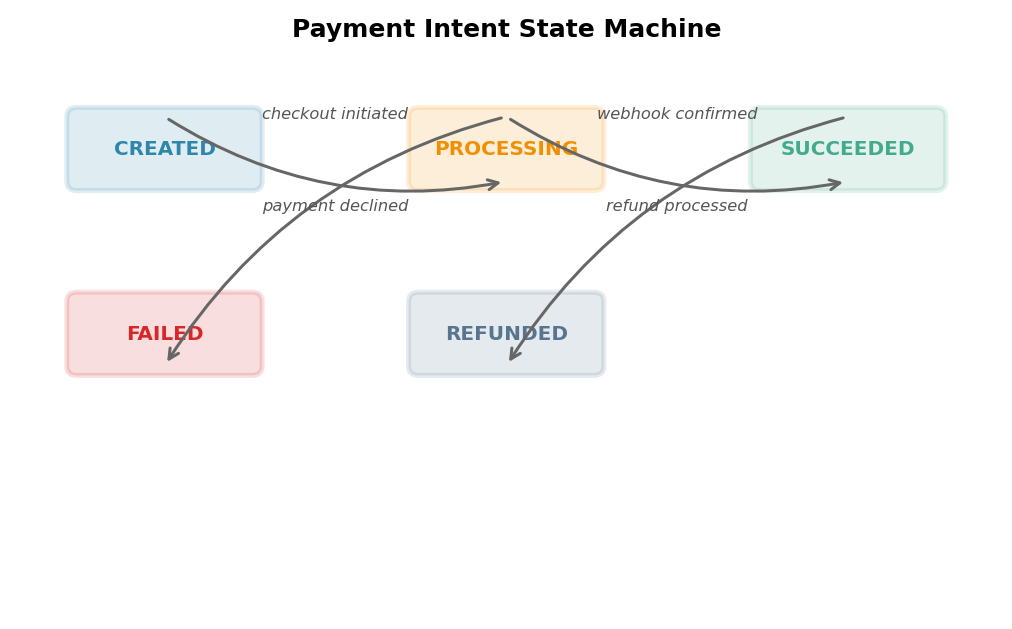
\includegraphics[width=0.65\textwidth]{images/statemachines/payment_intent_statemachine.png}
  \caption{Payment Intent State Machine}
  \label{fig:payment-statemachine}
\end{figure}

The \texttt{PaymentIntent} aggregate transitions through states: CREATED when the checkout session is initiated, PROCESSING while awaiting Stripe confirmation, SUCCEEDED upon confirmed payment, FAILED if the payment was declined or expired, and REFUNDED when a succeeded payment is refunded. Each transition is recorded as an immutable \texttt{PaymentEvent} in a separate event table, providing an audit trail for financial reconciliation.

\subsection{Reconciliation and Expiration Services}

Two scheduled services handle edge cases in the payment lifecycle:

\begin{description}
  \item[\textbf{ReconciliationService.}] Runs daily and retrieves all PaymentIntents in PROCESSING state older than 24 hours. It queries Stripe for the latest status of each associated Checkout Session and updates the local state accordingly, handling cases where the webhook was never delivered (e.g., network outage).
  \item[\textbf{ExpirationService.}] Runs hourly and expires Checkout Sessions older than 24 hours. This garbage-collects abandoned payment flows and releases any temporary holds on inventory or enrollment slots.
\end{description}

Both services are implemented as NestJS \texttt{@Cron} decorators with configurable cron expressions and are disabled in test environments.
